\section{Taller pellets: assembly feasibility}
The preceding frozen-boundary screen indicates a possible heat-lift direction, but it does not solve a changed cooler. Here the original 0.50 mm P/N legs are compared with a 0.60 mm \emph{coordinate proposal}; the 0.40 mm square section, 0.58 mm pitch, 29/11/4 couple allocation and bottom mounting datum are retained. The four 0.50 mm ceramic plates require cumulative translations of 0, 0.10, 0.20 and 0.30 mm, respectively. Source-coordinate arithmetic preserves nominal axial alignment of all 88 legs with both 0.035 mm solder interfaces and 0.16 mm$^2$ contacts. These are geometric construction checks, not a regenerated three-dimensional assembly or validated contact surfaces.

\begin{center}\small
\begin{tabular}{lrr}\toprule
Quantity & Original & Proposed \\ \midrule
Core height (mm) & 3.80 & 4.10 \\
Die top above header datum (mm) & 5.776 & 6.076 \\
Axial die--window separation (mm) & 3.874 & 3.574 \\
Total P/N lateral surface (mm$^2$) & 70.40 & 84.48 \\
Total P/N volume (mm$^3$) & 7.040 & 8.448 \\
Nominal interleg edge separation (mm) & 0.18 & 0.18 \\
\bottomrule\end{tabular}\end{center}
\noindent The 4.10 mm proposed stack exceeds the separate 3.80 $\pm$ 0.15 mm published product-height envelope; it is a synthetic design proposal, not a claim about a manufacturer's internal assembly. The die--window distance is an axial dimension and is not a collision or optical-clearance certification. The surface and volume changes are not a calculation of native gas conductance or gas volume.

\begin{figure}[htbp]\centering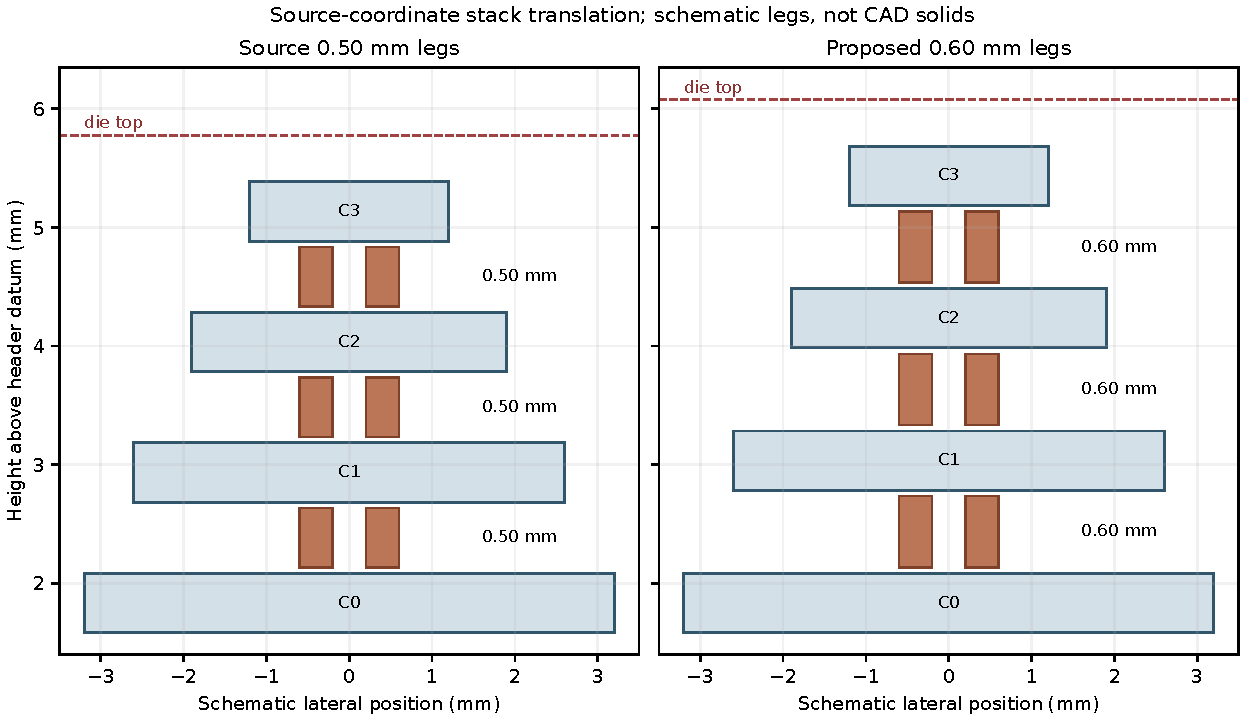
\includegraphics[width=.94\linewidth]{figures/v318_height_stack.pdf}\caption{Source-coordinate plate elevations and their proposed translations. Legs are schematic representatives; no candidate solids, contact mesh, copper paths or gas field are depicted.}\end{figure}

The formed-copper neutral paths 58 and 80 each need 0.10 mm additional rise; the three-foot return 88 needs 0.20 mm. Their source-fillet path lengths become 2.061, 2.071 and 3.906 mm, respectively, before any new interference or contact audit. The original detector bond wire cannot simply remain fixed: after moving its die endpoint 0.30 mm, only 0.065 mm rise remains below the original apex, less than the 0.15 mm bend radius. A raised-apex analytic path can be drawn, but remains unverified for assembly and clearances.

\textbf{Physical promotion and matched-power comparison remain stopped.} Candidate CAD, contacts, clearance checks, ceramic mappings, copper multiport and cavity exchange have not been regenerated and checked. No new detector temperature or package energy balance is reported. The original 3D electrical contact gate remains failed. A rebuilt assembly with independent checks is required before assessing any cooling benefit.
